\pdfminorversion=4
\documentclass[]{beamer}
\mode<presentation>
% Time-stamp: <2021-07-10 14:40:04 (jonahm)>

% beamer stuff
% Gives us the bottom line with all the goodies
\useoutertheme{infolines}
% Just the theme to use. Should be built into bemaer. Setting the
% height gets rid of a whole lot of whitespace
\usetheme[height=7mm]{Rochester}
\usefonttheme{serif}
% Usually beamer gives you navigation hyperlinks on the bottom
% right. I turned this off. It's annoying.
\setbeamertemplate{navigation symbols}{} 
% Makes my text boxes look pretty
\setbeamertemplate{blocks}[rounded][shadow=true] 
% Makes my bullet points 3d balls
\setbeamertemplate{items}[ball]

% Josh's packages
\usepackage{multimedia}
\usepackage{graphicx}

% Packages for me
\usepackage{amsmath,amssymb,latexsym,amsthm}
\usepackage[mathscr]{eucal}
\usepackage{mathrsfs}
\usepackage{verbatim}
\usepackage{braket}
\usepackage{listings}
\usepackage{xcolor}
% \usepackage[usenames,dvipsnames,svgnames,table]{xcolor}
\usepackage{fancybox}
\usepackage{animate}
% \usepackage{media9}
\usepackage{multicol}
\usepackage{mdframed}
\usepackage{hyperref}
%\usepackage{scalerel}
\usepackage[outline]{contour}
\contourlength{1.2pt}

% Macros

%Blackboard Bold
\newcommand{\R}{\mathbb{R}}
\newcommand{\Z}{\mathbb{Z}}
\newcommand{\N}{\mathbb{N}}
\newcommand{\Q}{\mathbb{Q}}
\newcommand{\A}{\mathbb{A}}
\newcommand{\E}{\mathbb{E}}
% other
\newcommand{\eval}{\biggr\rvert} %evaluated at
\newcommand{\myvec}[1]{\mathbf{#1}} % vectors for me
% total derivatives 
\newcommand{\diff}[2]{\frac{d #1}{d #2}} 
\newcommand{\dd}[1]{\frac{d}{d #1}}
% partial derivatives
\newcommand{\pd}[2]{\frac{\partial #1}{\partial #2}} 
\newcommand{\pdd}[1]{\frac{\partial}{\partial #1}} 
% Order operator
\DeclareRobustCommand{\orderof}{\ensuremath{\mathcal{O}}}

% braces
\newcommand{\paren}[1]{\left( #1 \right)}
\newcommand{\sqrbrace}[1]{\left[ #1 \right]}
\newcommand{\curlybrace}[1]{\left\{ #1 \right\}}
\newcommand{\inner}[1]{\paren{#1}}
\newcommand{\norm}[1]{\left| #1 \right|_2}

% g
\newcommand{\detg}{\sqrt{-g}}

% neutrinos
\newcommand{\eepsilon}{\epsilon} % energy
\newcommand{\fin}{f\in \{\nu_e,\nu_{\bar{e}},\nu_x\}}
\newcommand{\sign}{\text{sign}(f)}
\newcommand{\jnuf}{j_{\eepsilon,f}}
\newcommand{\etanuf}{\eta_{\eepsilon,f}}
\newcommand{\Inuf}{I_{\eepsilon,f}}
\newcommand{\chinuf}{\chi_{\eepsilon,f}}
\newcommand{\sigmanuf}{\sigma_{\eepsilon,f}}
\newcommand{\alphanuf}{\alpha_{\eepsilon,f}}
\newcommand{\numin}{\nu_{\text{min}}}
\newcommand{\numax}{\nu_{\text{max}}}


% tikz
\usepackage{tikz}
\usepackage{pgfplots}
\usetikzlibrary{arrows}
\usetikzlibrary{decorations.pathmorphing}
\usetikzlibrary{decorations.markings}
\usetikzlibrary{arrows.meta,bending}

% Keys to support piece-wise uncovering of elements in TikZ pictures:
% \node[visible on=<2->](foo){Foo}
% \node[visible on=<{2,4}>](bar){Bar}   % put braces around comma expressions
% 
% Internally works by setting opacity=0 when invisible, which has the 
% adavantage (compared to \node<2->(foo){Foo} that the node is always there, hence
% always consumes space plus that coordinate (foo) is always available.
% 
% The actual command that implements the invisibility can be overriden
% by altering the style invisible. For instance \tikzsset{invisible/.style={opacity=0.2}}
% would dim the "invisible" parts. Alternatively, the color might be set to white, if the
% output driver does not support transparencies (e.g., PS) 
% 
\tikzset{
  invisible/.style={opacity=0},
  visible on/.style={alt={#1{}{invisible}}},
  alt/.code args={<#1>#2#3}{%
    \alt<#1>{\pgfkeysalso{#2}}{\pgfkeysalso{#3}} % \pgfkeysalso doesn't change the path
  },
}

% some nice flowchart features
\tikzset{
    mynode/.style={rectangle,rounded corners,draw=black, top color=white, bottom color=yellow!50,very thick, inner sep=1em, minimum size=3em, text centered},
    myarrow/.style={->, >=latex', shorten >=1pt, thick},
    mylabel/.style={text width=7em, text centered} 
}  

% squigly arrow
\tikzset{zigzag it/.style={decorate, decoration=zigzag}}

% Color morphing arrow
\tikzset{colormorph/.style n args={3}{
    postaction={
    decorate,
    decoration={
    markings,
    mark=between positions 0 and \pgfdecoratedpathlength step 0.5pt with {
    \pgfmathsetmacro\myval{multiply(
        divide(
        \pgfkeysvalueof{/pgf/decoration/mark info/distance from start}, \pgfdecoratedpathlength
        ),
        100
    )};
    \pgfsetfillcolor{#3!\myval!#2};
    \pgfpathcircle{\pgfpointorigin}{#1};
    \pgfusepath{fill};}
}}}}

% define a really nice visible "purple"
\definecolor{gimppurple}{HTML}{AD26FB}
% a light grey
\definecolor{lightgrey}{HTML}{E0E0E0}
% for highlighting
\definecolor{deepblue}{rgb}{0,0,0.5}
\definecolor{deepred}{rgb}{0.6,0,0}
\definecolor{deepgreen}{rgb}{0,0.5,0}

% fonts
% Default fixed font does not support bold face
\DeclareFixedFont{\ttb}{T1}{txtt}{bx}{n}{12} % for bold
\DeclareFixedFont{\ttm}{T1}{txtt}{m}{n}{12}  % for normal

% Python style for highlighting
\newcommand\pythonstyle{\lstset{
language=Python,
basicstyle=\ttm,
otherkeywords={self},
keywordstyle=\ttb\color{deepblue},
emph={__init__},           
emphstyle=\ttb\color{deepred},
commentstyle=\ttfamily\color{deepred},
stringstyle=\color{deepgreen},
frame=tb,                     
showstringspaces=false        
}}

% Python environment
\lstnewenvironment{python}[1][]
{
\pythonstyle
\lstset{#1}
}
{}

\newcommand{\backupbegin}{
   \newcounter{finalframe}
   \setcounter{finalframe}{\value{framenumber}}
}
\newcommand{\backupend}{
   \setcounter{framenumber}{\value{finalframe}}
}

% Automatically generates section breaker slides
\AtBeginSection[]{
  \begin{frame}[plain]
  \vfill
  \centering
  \begin{beamercolorbox}[sep=8pt,center,shadow=true,rounded=true]{title}
    \usebeamerfont{title}\insertsectionhead\par%
  \end{beamercolorbox}
  \vfill
  \end{frame}
}

\title[nubhlight]{$\nu\texttt{bhlight}$ Overview}
% \subtitle{Models and Implications}
\author[J. Miller]{Jonah M. Miller}
\institute[LANL]{Los Alamos National Laboratory}
% \titlegraphic{\vspace{1cm}}
% \titlegraphic{\includegraphics[height=0.25\textheight]{3d_render}}
% \date[7/12/21]{ECT* Workshop}

\graphicspath{{figures/}}

\begin{document}

\begin{frame}[plain]
    \tikz [remember picture, overlay] 
    \node at ([xshift=2cm,yshift=-2cm]current page.west)
    {\includegraphics[width=0.25\textwidth,clip,trim={150 0 150 0}]{3d_render}};
    \tikz [remember picture, overlay] 
    \node at ([xshift=-2cm,yshift=-2cm]current page.east)
    {\includegraphics[width=0.25\textwidth,clip,trim={0 0 0 0}]{visit0006-gimp3}};
  \titlepage
\end{frame}

% \begin{frame}
%   \frametitle{Neutron Star Mergers: A 2+ Component Model}
%   \begin{columns}
%     \begin{column}{6cm}
%       \begin{center}
%         % \includegraphics[width=0.9\textwidth]{frames/betabin_000}
%         \animategraphics[width=0.9\textwidth,every=10,autoplay,loop,controls]
%         {5}{frames/betabin_}{000}{374}
%       \end{center}
%     \end{column}
%     \begin{column}{6cm}
%       \begin{center}
%         \resizebox{\columnwidth}{!}{
%           \begin{tikzpicture}
%             \coordinate (origin) at (0,0);
%             \pgfmathsetmacro{\dbx}{0.5}
%             \pgfmathsetmacro{\dby}{0.05}
%             \pgfmathsetmacro{\dex}{2.}
%             \pgfmathsetmacro{\dey}{0.25}
%             \pgfmathsetmacro{\dcc}{2.1}
%             \pgfmathsetmacro{\tcx}{5.0}
% 
%             \foreach \i in {-1,1}
%             {
%               \fill[ball color=blue] (0, \i*2.9) ellipse (2 and 3);
%             }
% 
%             \foreach \i in {-1,1}
%             {
%               % disk
%               \fill[color=orange]
%               (\i*\dbx,\dby) -- (\i*\dex,\dey)
%               .. controls (\i*\dcc,0) .. (\i*\dex,-\dey)
%               -- (\i*\dbx,-\dby) -- cycle;
% 
%               % tidal ejecta
%               \fill[color=red] (\i*\tcx,0) ellipse (0.75 and 1.5);
%             }
% 
%             % viewing
%             \draw[dashed,ultra thick,black] (origin) -- (5,4);
%             \draw[dashed,ultra thick,black] (origin) -- (3,6);
%             \fill[color=gray,opacity=0.5] (origin) -- (5,4) -- (3,6) -- cycle;
%             \node[right,align=left] at (3.5,5)
%             {\Large $\sim$ GW170817\\ \Large Viewing angle};
% 
%             % bh
%             \shade[ball color=black] (origin) circle (0.25);
% 
%             % text
%             \draw[<-,red, ultra thick] (\tcx,1.5)
%             -- ++(0.,0.5) -- ++(0.5,0)
%             node[right,align=left]
%             {\Large \color{red}$n$-rich\\\Large Tidal Ejecta\\ \Large $\sim 5\times 10^{-3}M_{\odot}$};
% 
%             \draw[<-,blue, ultra thick] (0,6) -- ++(0,1) -- ++(-2,0)
%             node[left,align=right]
%             {\Large \color{blue}$n$-poor\\\Large disk wind\\\Large $\sim 10^{-2}M_{\odot}$};
% 
%             \draw[<-,orange, ultra thick] (\dex,-\dey)
%             -- ++(2,-3) -- ++(1,0)
%             node[right,align=left]
%             {\Large \color{orange}Disk\\\Large $\sim 10^{-1}M_{\odot}$};
% 
%             \draw[<-,black, ultra thick] (-0.25,-0.25)
%             -- ++(-2,-3) -- ++(-1,0)
%             node[left,align=right]
%             {\Large \color{black}Black Hole\\ \Large $\sim 2 M_{\odot}$};
%           \end{tikzpicture}
%         }
%       \end{center}
%     \end{column}
%   \end{columns}
%   \begin{tiny}
%     Co-design summer school, 2016
%   \end{tiny}
% \end{frame}
% 
% \begin{frame}
%   \frametitle{The August 2017 Disk (Miller et al., 2019)}
%   \begin{center}
%     % \includegraphics[height=0.475\textheight]{gw170817disk_Ye_close/frame_0831} \\
%     % \includegraphics[height=0.475\textheight]{gw170817disk_Ye_far/frame_0831} 
%     \animategraphics[height=0.475\textheight,every=5,autoplay,loop,controls=off]
%     {10}{gw170817disk_Ye_close/frame_}{0001}{0837} \\
%     \animategraphics[height=0.475\textheight,every=5,autoplay,loop,controls=off]
%      {10}{gw170817disk_Ye_far/frame_}{0001}{0837} 
%   \end{center}
%   %\textbf{JMM}+, in prep.
% \end{frame}

\begin{frame}
  \frametitle{Ingredients In Kilonova Disk Modeling}
  \begin{itemize}
  \item General relativity
    \begin{itemize}
    \item Rotating black hole spacetime
    \end{itemize}
  \item Plasma physics
    \begin{itemize}
    \item Ideal magnetohydrodynamics
    \end{itemize}
  \item Nuclear physics
    \begin{itemize}
    \item Hot gas treated as being in nuclear-statistical equilibrium via \textbf{equation of state}
    \item Cooling outflow treated in postprocessing via \textbf{nuclear reaction networks}
    \end{itemize}
  \item Radiation physics
    \begin{itemize}
    \item Material is opaque to photons, can be incorporated in plasma physics
    \item Material \textit{not} opaque to \textbf{neutrinos}.
    \item Neutrinos can \textit{change the composition of the
        material} by converting neutrons to protons and vice versa.
    \end{itemize}
  \end{itemize}
\end{frame}

\begin{frame}
  \frametitle{Ingredients in Kilonova Disk Modeling}
  \begin{itemize}
  \item Mass conservation:
    \begin{small}
      \begin{displaymath}
        \partial_t \paren{{\color{red}\detg}\rho u^t}
        + \partial_i\paren{{\color{red}\detg}\rho u^i} = 0
      \end{displaymath}
    \end{small}
  \item Momentum and Internal Energy Conservation:
    \begin{small}
      \begin{displaymath}
        \partial_t\sqrbrace{{\color{red}\detg} \paren{T^t_{\ \nu} + \rho u^t \delta^t_\nu}}
        + \partial_i\sqrbrace{{\color{red}\detg}\paren{T^i_{\ \nu} + \rho u^i \delta^t_\nu}}
        = {\color{red}\detg} \paren{T^\kappa_{\ \lambda} {\color{red}\Gamma^\lambda_{\nu\kappa}} + {\color{blue}G_\nu}}
      \end{displaymath}
    \end{small}
  \item Magnetic Fields
    \begin{small}
      \begin{displaymath}
        \partial_t \paren{{\color{red}\detg} B^i}
        - \partial_j \sqrbrace{{\color{red}\detg}\paren{b^ju^i - b^i u^j}}
        = 0
      \end{displaymath}
    \end{small}
  \item Composition
    \begin{small}
      \begin{displaymath}
        \partial_t\paren{{\color{red}\detg}\rho Y_e u^t}
        + \partial_i\paren{{\color{red}\detg}\rho Y_eu^i}
        = {\color{red}\detg} {\color{blue}G_{\text{ye}}}
      \end{displaymath}
    \end{small}
  \item Neutrino Transport
    \begin{small}
      \begin{displaymath}
        {\color{red}\frac{D}{d\lambda}}\paren{\frac{h^3\Inuf}{\eepsilon^3}}
        = \paren{\frac{h^2{\color{blue}\etanuf}}{\eepsilon^2}}
        - \paren{\frac{\eepsilon {\color{blue}\chinuf}}{h}} \paren{\frac{h^3\Inuf}{\eepsilon^3}},
      \end{displaymath}
    \end{small}
  \end{itemize}
\end{frame}

\begin{frame}
  \frametitle{The Equations of Special-Relativistic Hydrodynamics}
  \begin{itemize}
  \item Assumptions:
    \begin{itemize}
    \item Minkowski spacetime: $g_{\mu\nu} = \text{diag}(-1, 1, 1, 1) \Rightarrow \sqrt{-g} = 1$
    \item Radiation, composition, and magnetic fields neglected
    \end{itemize}
  \item Mass conservation:
    \begin{small}
      \begin{displaymath}
        \partial_t \paren{\rho u^t} + \partial_i\paren{\rho u^i} = 0
      \end{displaymath}
    \end{small}
  \item Momentum and Internal Energy Conservation:
    \begin{small}
      \begin{displaymath}
        \partial_t\sqrbrace{\paren{T^t_{\ \nu} + \rho u^t \delta^t_\nu}}
        + \partial_i\sqrbrace{\paren{T^i_{\ \nu} + \rho u^i \delta^t_\nu}}
        = 0
      \end{displaymath}
    \end{small}
  \end{itemize}
\end{frame}  

\begin{frame}
  \frametitle{Einstein Summation and Abstract Index Notation}
  \begin{itemize}
  \item Repeated indices are summed:
    $$a_i b^i = \sum_{i=1}^3 a_i b^i$$
  \item Greek indices range from 0 to 3, Latin from 1 to 3.
  \item Index up or down indicates row or column
    vector---contravariant or covariant. Transformation between them
    enabled by multiplication by \textit{metric}:
    $$a_\mu = g_{\mu \nu} a^\nu$$
    for $g_{\mu\nu} = \eta_{\mu\nu} = \text{diag}(-1, 1, 1, 1)$.
  \item $g^{\mu\nu}$ is matrix inverse of $g_{\mu\nu}$.
  \item Later, $g$ will be more general. $|g| < 0$ always.
  \end{itemize}
\end{frame}

\begin{frame}
  \frametitle{The Four-Velocity $u^\mu$}
  \begin{itemize}
  \item Describes direction of travel in \textit{space-time}.
  \item For matter (but not radiation),
    $$u^\mu u_\mu = -(u^0)^2 + u_i u^i = -1$$
  \item For this reason, convenient to work with
    $$v^i = \frac{u^i}{u^0}\text{ s.t. } u^0 = \sqrt{1 + v^i v_i}$$
  \item Turns out $u^0$ related to important quantity the \textit{Lorentz factor}, $W$. More generally,
    $$W = \sqrt{1 + v^i v_i}\text{ and }u^0 = W/\alpha$$
    but we'll get there.
  \end{itemize}
\end{frame}

\begin{frame}
  \frametitle{The Energy-Momentum Tensor}
  \resizebox{12cm}{!}{
    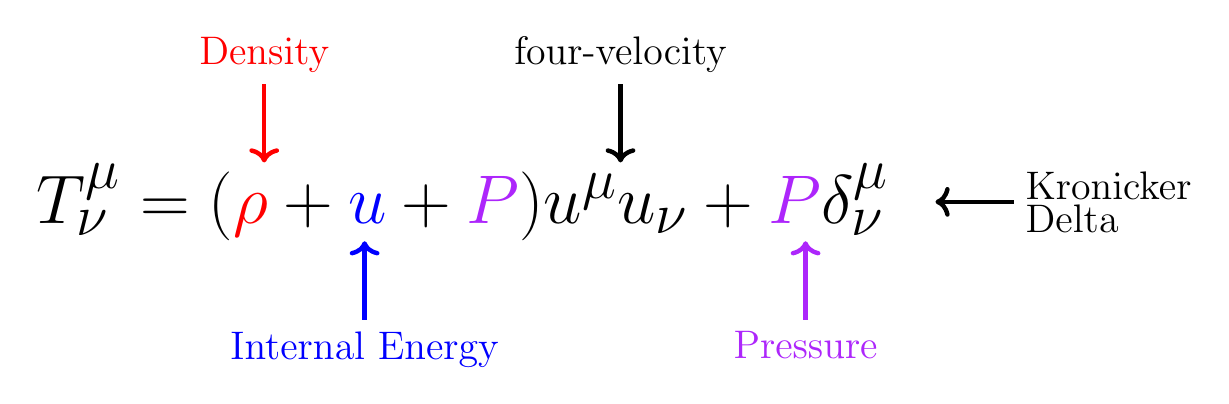
\begin{tikzpicture}
      \coordinate (origin) at (0, 0);
      \node[align=center] at (origin)
      {\Huge $T^\mu_\nu = ({\color{red}\rho} + {\color{blue}u} + {\color{gimppurple}P}) u^\mu u_\nu + {\color{gimppurple}P} \delta^\mu_\nu$};
      \draw[ultra thick, <-] (2,0.5) -- ++(0, 1) node[above,align=center] {\Large four-velocity};
      \draw[ultra thick, <-] (6, 0) -- ++(1, 0) node[right,align=left] {\Large Kronicker\\ \Large Delta};
      \draw[gimppurple, ultra thick, <-] (4.35, -0.5) -- ++(0,-1)  node[below,align=center] {\Large Pressure};
      \draw[blue, ultra thick, <-] (-1.25, -0.5) -- ++(0, -1) node[below,align=center]{\Large Internal Energy};
      \draw[red, ultra thick, <-] (-2.525, 0.5) -- ++(0,1) node[above,align=center]{\Large Density};
    \end{tikzpicture}
  }
\end{frame}

\begin{frame}
  \frametitle{Now We can Read the Conservation Laws}
  \begin{itemize}
  \item Mass conservation:
    \begin{small}
      \begin{displaymath}
        \partial_t \paren{\rho u^0} + \partial_i\paren{\rho u^i} = 0
      \end{displaymath}
    \end{small}
  \item Momentum Conservation
    \begin{small}
      \begin{displaymath}
        \partial_tT^0_{\ j} + \partial_iT^i_{\ j} = 0
      \end{displaymath}
    \end{small}
  \item Momentum and Internal Energy Conservation:
    \begin{small}
      \begin{displaymath}
        \partial_t\sqrbrace{\paren{T^0_{\ 0} + \rho u^0}}
        + \partial_i\sqrbrace{\paren{T^i_{\ j} + \rho u^i}}
        = 0
      \end{displaymath}
    \end{small}
  \item Where
    $$\partial_t = \frac{\partial}{\partial t}\text{ and }\partial_i = \frac{\partial}{\partial x^i}$$
  \item $T^0_{\ \nu}$ called \textit{conserved} variables. $T^i_{\ nu}$ called \textit{fluxes}.
  \end{itemize}
\end{frame}

\begin{frame}
  \frametitle{Primitive vs Conserved variables}
  \begin{itemize}
  \item It is convenient to work in two sets of variables.
  \item Together, $\rho$, $u$, $v^i$, and $P$ make up the
    \textit{primitive} variables. Sometimes temperature $T$ also
    included.
  \item The conserved variables are the $\mu=0$ components of
    $T^\mu_\nu$, and Baryon number, $\rho u^0$.
  \item Conserved variables can easily be computed from primitives
    algebraically, but the opposite is not the case. The inversion is
    often not known analytically and must be computed numerically.
  \item The Euler equations are insufficient to determine pressure and
    temperature. An \textit{equation of state} must be assumed that
    relates, e.g., pressure to density and energy. For example, the
    \textit{ideal gas} equation of state:
    $$P = (\gamma - 1) u$$
    which we will assume for now.
  \end{itemize}
\end{frame}

\begin{frame}
  \frametitle{Other Important Quantities}
  \begin{itemize}
  \item Linearizing the above equations leads to a wave equation for
    waves that travel at specific speeds.
  \item These are \textit{sound waves} with speed
    $$c_s = \sqrt{\frac{\partial P}{\partial \rho}}$$
  \item Other thermodynamic derivatives such as specific heat
    $$C_v = \frac{\partial (u/rho)}{\partial T}$$
    can also be relevant.
  \end{itemize}
\end{frame}

\backupbegin

\backupend

\end{document}